\documentclass{report}

\usepackage[pdftex]{graphicx}
\usepackage{parskip}


\begin{document}
\title{SPRS: The Simplified Packet Relay System}
\author{Kenneth Finnegan}
\maketitle

\begin{abstract}
The Automatic Packet Reporting System (APRS) is an amateur radio packet 
network that has evolved over the last several decades in tandem with, 
and then arguably beyond, the lifetime of other VHF/UHF amateur packet
networks, to the point where it is one of very few packet networks left
on the amateur VHF/UHF bands. This is proving to be problematic due to
the loss of institutional knownledge as older amateur radio operators who
designed and built APRS and other AX.25-based packet networks relieve 
themselves of the hobby or pass away. The purpose of this document is to 
collect and currate a sufficient body of knownledge to ensure the 
continued usefulness of the APRS network moving on, and re-examining 
the engineering decisions made during the network's evolution to look for
possible improvements and document deficiencies in the existing network.
\end{abstract}

\tableofcontents



\chapter{Introduction}

The Automatic Packet Reporting System (APRS) is an amateur radio packet
network designed to provide each participating node a local view of the 
tactical environment based on each node beaconing it's current status
and advertising any other local resources known to exist.

Exactly what types of resources should be advertised on a local APRS
network is left to the discretion of the local network coordinators, but
a typical APRS network would advertise information such as:
\begin{itemize}
\item The location of amateur radio operators and what frequencies they are using for voice communications.
\item The location, frequency, and access information for voice repeaters
\item The location and status of APRS digital repeater nodes
\item The location and access information for other packet networks such as BBSes, Winlink nodes, or open Internet access points.
\item The location and status of useful facilities such as rest stops, resupply points for food/water, etc.
\item Telemetry from sensors such as weather stations or remote site monitoring (i.e. battery voltage at solar sites)
\end{itemize} 

\section{Goals of This Document}

One of the greatest failings of amateur packet radio is the lack of definitive
collections of documentation on the complete protocol stacks currently used in 
networks such as APRS. This is understandable as the task of documenting a 
system as complex as APRS is momumental and requires digging through decades of 
relevant standards, magazine articles, and personal diatribes made by amateurs
infulential in the field.

The body of this document is divided into three sections loosely based on the 
three lowest layers of the OSI seven layer network model. Many portions of the APRS
protocol stack
pre-date the OSI model, and maintaining clean separation of layers even in 
contemporary protocols is challenging, so the lines drawn in this document should
be viewed with a level of forgiveness by the reader. More importantly, these three
layers are drawn to aid future work on experimenting with physical modulation 
and data link protocols underneath the APRS packet application.

While some of these differentiations already exist in the standing literature,
this document isn't holding itself bound to the existing implicit conventions.
One example is the likely controversial separation made between Bell 202 and 
AX.25 where I (the author?) have gone as far as to
remove the Frame Checksum (FCS) from AX.25 packets all together and place them
instead in the Bell 202 frame, motivated by the fact that AX.25 packets are moved
across other physical channels such as KISS without the required FCS.

\section{History of APRS}

APRS was created as an evolution of the AX.25 packet networks
built throughout the amateur community during the 1980s and 1990s and 
the Connectionless Emergency Traffic System (CETS) built by 
Bob Bruninga during the early 1980s to map Navy position reports.

Near-ubiquitious access to the Internet caused the decline in local BBS 
systems and AX.25 TCP/IP networks during the 1990s, but APRS has 
continued to enjoy a growing userbase due to it filling a unique 
application of amateur packet radio to local short-lived communication.

APRS supports basic communication between stations via node to node 
text messages and comment field status updates, but should not be 
considered a communications network to an end, but a way to be made aware
of the other assets in the local area made available to support amateur 
radio operations.

Due to the fact that APRS is built upon the relatively slow 
1200bps AX.25 VHF packet
network and the channel sharing concepts developed for the ALOHAnet at
the University of Hawaii, the amount of 
traffic and the number of stations that it is possible to successfuly 
support on a single regional network is severly limited. 
A tyical APRS network is considered successful if a single node
can use it to discover the 60 closest other assets on the network in a
10-30 minute time frame. Trying to advertise information beyond this
``ALOHA circle" consisting of the 60 closest stations exceeds the 
operational objective of the APRS network and usually proves to only be 
detrimental to the network and other users as network throughput is 
consumed by advertisements for 
resources beyond the radius of interest for the local operator.


\input{networklayers.tex}
\part{OSI Layer 1 --- Physical}

The physical layer of APRS defines the different signalling methods used
to transport datalink layer packets from one node to another across one of
the several physical channels typically used in the APRS network.


\chapter{Bell 202 on RF}

The most common layer 1 used for APRS on RF is a variant of the
Bell 202 audio frequency shift keyed (AFSK) modem transmitted via 
FM VHF radios. In North America, the primary frequency of operation is
144.390MHz, but differs by country based on local band limitations.

Bell 202 was originally  based on switching between 1200Hz and 2200Hz tones to
represent a binary one or zero respectively. Due to Amateur radio operators
using Bell 202 as a physical layer below AX.25, which ultimately derived 
from HDLC, the original 1200Hz mark and 2200Hz space symbols are not used;
the layer 2 data stream is encoded using 
non-return to zero, inverted (NRZI),
which requires zeros in the original bit stream to be encoded as a change
between 1200Hz and 2200Hz and ones to be encoded as transmitting the same
symbol during the next symbol period as during the prior.

\section{Stages of a Bell 202 Transmission}

Channel idle state; string of zeros for clock sync

At least one flag octet 0x7E

AX.25 UI frame with bit stuffing

Frame Check Sum; 16 bit CCITT CRC

At least one flag octet 0x7E

Release of channel or an additional AX.25 frame and flag. 

\section{Baseband Performance of Bell 202 Modems}

TODO No FEC is severe limitation

TODO Emphasis / deemphasis problem is unsolvable

TODO Define Basic 3002 phone channel as good benchmark

\section{Carrier Sense Multiple Access}

Since amateur Bell 202 is a half duplex modulation traditionally using FM voice 
transceivers, one of the challenges to packet radio is avoiding multiple stations
transmitting on the same channel at once. Other derivatives of ALOHAnet, such as 
the original half duplex 10Mbps Ethernet, have the advantage that transmitters can
at least sense when a collision has taken place and use that information to abort
the transmission of the rest of the frame.

Throughout the history of APRS, there has been several debates as to the implications
of CSMA algorithms and primarily the need for one at all versus an entirely 
stocastic channel access method. The argument follows that the majority of 
channel contention is between multiple clients trying to reach a single digipeater
across what's called a split horizon, where each of the clients can hear and be heard
by the digipeater, but are entirely unaware of each other. In these types of instances,
even an optimal CSMA algorithm will never correctly cause one of the stations to hold 
off until the end of the other's transmission due to the needed information being
entirely unavailable.

Besides the degenerate case of ignoring the current channel status completely when 
deciding to transmit a pending frame, there are two major algorithms used for CSMA;
DWait and P-persistent.

DWait is a deterministic algorithm where each station is assigned a fixed
``quiet time" after the end of another tranmission before they will begin a locally
pending tranmission. This lends itself well to very carefully designed networks
where the relative priority of each station is known and a corresponding DWait time
is set for each station where a shorter DWait will always gain the channel over a longer
one. The requirement for the network to have an overarching design doesn't lend itself
well to the national APRS network, but could be applied effectively for localized 
portions of the APRS network and for ``insular" networks built for special events or
private groups of amateurs.

P-persistent is a statistical algorithm with two variables: the slot time, and the
probability that a station should transmit at the beginning of a slot. The slot time
should presumably be set to as short of a time interval during which a station can
reliabily identify another station as transmitting before beginning its own transmission,
and the P value for how likely a station is to transmit should be set based on the 
number of other stations with pending traffic attempting to gain the channel.

TODO Table of typical mobile radio tx-rx and rx-tx changeover times.
TODO The typical 100ms slot time seems to be much too short.

\chapter{KISS}

KISS (``Keep It Simple, Stupid") is a protocol originally presented by 
Mike Chepponis, K3MC and Phil Karn, KA9Q at the 6th ARRL Computer Networking
Conference in Redondo Beach, CA in 1987 as an extension to the Serial Line 
Internet Protocol (SLIP) described in RFC 1055 allowing for in-band signalling from 
the host to the Terminal Node Controller (TNC) to enable setting modem 
configuration parameters. 

During the early 1980's, the expectation was that the TNC would be handling 
the entire packet protocol stack up to the final presentation to the user, which
could conceivably be done using a dumb terminal such as a VT100 or line printer 
and a keyboard. 
Once personal computers became affordable in the late 1980's, the expectation that
the entire application stack would run on the embedded TNC became severely limiting
and KISS emerged as the solution to expose the modems inside TNCs via 
an eight bit clean interface.

TODO Describe typical application of KISS in node.

TODO Being 8 bit clean is a huge advantage.

TODO Doesn't allow for TNC to host message passing

\chapter{Bell 103 and PSK63}

TODO Mention the two main HF modes. 


\part{OSI Layer 2 --- Data Link}
\label{part:datalink}

\chapter{TNC2 Monitor}

The TNC2 was a terminal node controller developed by TAPR which
quickly became the definitive TNC in the amateur packet network.
This popularity meant that it enjoyed becoming the de-facto 
standard for many of the commands and interfaces involving 
TNCs.

One of the de-facto standards solidified by the TNC2 is the text
representation of AX.25 packets, which the TNC2 used in what it
called ``monitor mode." This mode asked that the TNC print 
every packet it received via RF to the local console such that
users can see and monitor the other AX.25 traffic on the channel.
While the TNC2 monitor mode does not capture the entire state of 
an AX.25 header, APRS uses so little of the header (as discussed in
the AX.25 chapter) that the TNC2 markup proved sufficient as the 
format used to pass APRS packets throughout the APRS-Internet System
backbone created to aggregate APRS traffic online.

Each packet must consist of a source address, a destination address,
an optional list of digipeaters, and the packet payload.
The source and destination calls are separated by a right chevron,
followed by a comma separated list of digital repeaters, and finally
terminated by a colon before the higher layer payload.

The digipeaters are listed in sequential order, and an asterisk
is appended to at least the last digipeater in the 
routing path that has already processed and re-transmitted the packet.
Some implementations of the TNC2 monitor mode append the ``consumed"
asterisk to every used digipeater in addition to the last one,
which semantically makes no difference due to digipeaters
being consumed in a strictly monotonic order.

TODO I think the APRS-IS uses the later format.

SRCCALL\textgreater{}DSTCALL,DIGI*,DIGI:,Packet payload


\chapter{AX.25}

AX.25 is the amateur radio derivative of CCITT X.25 that was designed during the early 1980's 
as the primary data link protocol used by amateur packet networks.
The AX.25 specification has been maintained by the Tucson Amateur Packet Radio (TAPR) 
organization until its latest release, Version 2.2 in July of 1998. 

The most significant difference between AX.25 and the original X.25 protocol lies
in the hardware addesses used by AX.25 based on each station's FCC issues callsign. 
Each node is addresses by their FCC callsign plus an additional 4 bit 
secondard station identifier (SSID), which allows each licensee to maintain and operate 
up to 16 stations in each packet namespace.

\section{FCC Identification Requirements}

One of the advantages of using a station's FCC callsign as part of the addressing protocol
is that it additionally fulfills the FCC requirement to identify every transmitting station
every ten minutes per Title 47 CFR \S97.119. \S97.119 is unfortunately vague and archaic as
to the exact requirements for this identification every ten times during a transmision. No
definitive judgements were found by the author as to 
the actual legal implications of the following protocol
for identifying operating stations, and this section must not be interpreted as any form of
legal advice on a station's legal identification requirements.

Source stations are identified during every transmission by including an ASCII representation
of their FCC callsign in the source address field of their AX.25 frames. 
Each Digipeater that subsequentlu handles this third party traffic may identify by appending 
their callsign to the packet's routing path and ensuring that it is the last valid FCC callsign
marked as ``consumed" as will be explained in section~\ref{subsec:ax25RoutingPath}.

The two exceptions to this rule are what are called non-trace digipeaters which do not
append their callsign to a packet's routing path and any station which uses a tactical callsign
instead of their FCC-issued callsign. Tactical callsigns are often used for packet stations to
give them more meaningful addresses than their control operator's callsign. One example of where
tactical callsigns are often used is events where APRS is used to track support vehicles that 
already have tactical callsigns issued to their voice operators, such as ``SAG-3" or ``CHASE-1."
Since these stations do not use their FCC callsign as part of their AX.25 address,
these stations do need to somehow ensure that they transmit their callsign 
at least once every ten minutes while operating, which
may be accomplished by including the control operator's callsign in the comment text of an 
originating APRS beacon.

\section{Header Format for APRS}

A very limited subset of the complete AX.25 protocol is used by APRS due to APRS 
deliberately avoiding the use of any of the connected or control modes of AX.25. This 
means that any AX.25 protocol stack used for APRS need only support unconnected information (UI)
frames per the AX.25 specification.

\begin{figure}
	\centering
	\includegraphics[width=1.0\textwidth]{src/dia/ax25ui}
	\caption{AX.25 UI Packet Format}
	\label{ax25uiformat}
\end{figure}

\subsection{TNC Description / Destination Address}

Traditional AX.25 traffic is usually directed at a single station, which would be indicated by 
a packet's destination address. Since APRS is strictly a one-to-many network protocol at layer 3, this field
is not needed for APRS and has been overloaded for several different applications.

The most popular application for this field is to be used as a tracker identifier, where a
six character identifier is allocated from the APRS Working Group to identify a specific 
APRS TNC and firmware version. Experimental trackers which have not yet received a tracker ID
should use the APZ??? identifier.

\subsection{Source Address}

The source address is the FCC or tactical callsign used by the beaconing APRS station, with an 
additional SSID appended to the station, which may range from zero to 15. Source addresses must 
be at least three characters long, and may not be any longer than six. Stations using AX.25 
over RF are limited to the SSID's of -0 to -15 due to AX.25's binary format, 
while stations using alternative data link transports may use any 
two alphanumeric characters for their SSID.

\subsection{Routing Path}
\label{subsec:ax25RoutingPath}

The AX.25 routing path is an optional variable-length field consisting of an ordered list of
digipeaters which should process and retransmit the considered packet. Should a station not
require the use of this field, it can be completely omitted and the end-of-path bit should be
set on the source address field. The path must consist of an integer number of seven octets.

The original AX.25 version 2.0 spec allowed for anywhere from zero to eight digipeaters to
be included in an AX.25 frame. Unfortunately, due to the unreliable nature of amateur 
packet radio, packets with a routing path requesting as many as eight hops would rarely be 
successfully delivered to the end station, so the version 2.2 specification for AX.25 was
rewritten limiting the number of requested digipeaters to two with the argument that packets
traveling beyond two hops should be handled by a higher layer protocol than AX.25.
This limitation, and the unclear figure 3.1 which indicates that only zero or two digipeaters
are allowed, are both ignored by APRS, which allows the original eight digipeater path, but
users are strongly discouraged from using beyond three hops on the national network.

\subsection{Control Flags}

The Control Flag octet indicates what type of AX.25 frame the considered packet is. 
Since APRS stictly uses only Unconnected Information (UI) frames, this field must
contain the value of 0x03.

\subsection{Protocol IDentifier}

The Protocol IDentifier (PID) field is normally used to identify the layer three protocol
being transported by AX.25. TAPR has reportedly stopped processing requests for new PID
values to be issued to new layer 3 applications of AX.25 \cite{millernopid}, 
so APRS uses the value of
0xF0 indicating that no layer 3 protocol is in use.

\subsection{Information Field}

The rest of the AX.25 frame contains the APRS payload in what is called the Information field.
The end of the Information field is indicated by the layer 1 modulation, which is traditionally
the Bell 202 FCS and 0x7E flag.



\chapter{Digital Repeater Routing Behavior}

An integral part of APRS is the huge array of digital repeaters deployed throughout the network.
The job of the digipeaters is to receive, process, and selectively retransmit packets from other 
stations in the network to improve network coverage and each station's effective range.
Originally, since AX.25 was used almost exclusively for static networks, it was valid that
the networks relied on the concept of manually constructing the exact string of digipeater hops
between two stations. When one of these digipeaters subsequently went down, a new route would 
need to be found between the two stations.

One of the large inovations of APRS was that these literal routing paths be replaced with 
well-known universal aliases for digipeaters such that a single node could move from area to
area and the local infrastructure would still support the same requested routing behavior.

\section{RELAY,WIDE}

The original conception of APRS included several aliases, but the most important were RELAY
and WIDE. Digipeaters were divided into two categories depending on if they were high-level
(on the top of large towers, mountain tops, etc.) or low-level (primarily sub-40' home installs).

Low-level ``fill-in" digipeaters are needed to assist low-power moving trackers in reaching the
primary high-level digipeater network where it would be possible to be heard by other stations.
Without these fill-in repeaters, lower power beacons would be lost in the noise and never reach the 
network at large. Therefore, trackers that need this help would begin their routing path with RELAY.

The high-level digipeaters that consist the major portion of the network coverage in terms of area
would respond to the alias of WIDE, in addition to the alias of RELAY such that if a tracker got
lucky and happened to be decoded by one of the high level digis it wasn't punished for first requesting 
help from a lower-level digi.

This RELAY for low-level and both RELAY and WIDE alias for high-level digipeater concept worked well
because the existing packet hardware at the time natively supported configuring these aliases, but
became increasingly problematic as the APRS network grew and became higher density. Each digipeater
could not verify that they had already retransmitted a beacon, so single packets would ``ping-pong" 
between digipeaters repeatedly until the entire path was finally consumed.

To solve this, a new digipeater behavior was implemented where each digi would keep a log of
all the packets it had retransmitted in the last 30 seconds based on the source callsign and 
packet contents (TODO verify the exact fields needed for dedup behavior). Therefore, when a digipeater 
hears an echo of an already digipeated packet, it will correctly ignore it and not generate more
redundant traffic on the APRS channel.

\section{WIDEn-N}

At the same time as the development of the deduplication concept, a new alias of WIDEn-N was 
developed with the goal of shortening AX.25 headers. A typical packet requesting three hops through
WIDE digipeaters would construct a routing path of ``WIDE,WIDE,WIDE," which would cause the 
AX.25 header to become 21 bytes longer than the minimum 16. The idea of WIDEn-N was to replace this
three hop path with a single alias of ``WIDE3-3," where the first number indicates the originally
requested number of hops and the second number the number of remaining hops. Therefore, as a packet
with an original path of "WIDE3-3" moved through digipeaters, each digipeater would rewrite the path 
to be ``WIDE3-2," ``WIDE3-1," and finally ``WIDE3-0*" at which point the path would be completely 
consumed and should no longer be digipeated.

While this was a sound design at the time, a failure in the implementation of this alias in one of
the more popular firmware revisions of Kamtronics TNCs meant that the deduplication algorithm used to
prevent packet echos from bouncing between digipeaters was not applied between the WIDEn-N and the 
original RELAY alias. Excessive cost to purchase new firmware ROMs from Kamtronics meant that much
of the network had no choice but to find a technical workaround to this firmware bug.

The lasting solution to this issue was proposed by Stephen Smith where the alias of RELAY would be
replaced by an alias of WIDE1-1, which allowed the Kamtronics' TNCs to use their deduplication
algorithms while preserving a literal alias to be used by the lower level digipeaters, many of which
did not and never would support the WIDEn-N alias concept. Low-level digis would respond to WIDE1-1, 
while higher level digis would respond to all permutations of WIDEn-N.

The only shortfall with this proposal to repurpose WIDE1-1 as a replacement for RELAY was that it
left no proper way to request a single hop from high-level digipeaters while excluding the low-level
digis not needed by stationary or high power trackers. The clever solution was to recommend that single
high-level hops be requested by the path of ``WIDE2-1," which literally means that the original tracker
requested two hops and that only one of them is left, which violates the original spirit of the leading
number in the alias but functionally yields the desired behavior.

\section{Digipeater Levels}

TODO This is where I flat out contradict the existing standard?



\part{OSI Layer 3 --- Network}

\chapter{APRS}

\chapter{Node Beaconing Behavior}

Due to the fact that APRS is a source-routed protocol, most of the decisions as
to how often a station should send traffic and how far that traffic should
travel are allowed to be made by that originating station. 
The existing specification for the protocol hardly touches on this issue, 
while a great deal of time and energy is spent on the development forums 
bemoaning specific examples of misbehaving members of the network.
The two major parameters under the source node's control that are considered
here are the frequency of beaconing and the routing path used for each beacon.

Being a source-routed protocol does fundamentally introduces a
moral hazard in the network. For each node in the network to enjoy the
most benefit from the network, they would want to beacon as often as possible 
with the longest path allowed by the network.
It is only by mutual trust, respect, and education that this 
logic isn't universally followed and the network is not grossly oversubscribed
in the self-interest of every individual network node. 
Unfortunately, the most popular documentation on APRS fails to stress the 
importance of correctly configuring nodes in the best interest for the network
at large, and rarely gives any concrete guidance on what values should typically
be used when configuring various types of network nodes.


\section{Beaconing Algorithms}

For each APRS node with information available for the network,
a local decision needs to be made as to when that information will best 
serve the local network and should be transmitted. This is rarely a trivial 
decision, and one that could warrent much more creative and application or data
specific solutions than the ones presented here, which should be considered 
the typical minimum of most popular APRS trackers. The only datum considered 
in this paper is that of a mobile node's position, but these algorithms would
likely extend to most other user applications of APRS.

\subsection{Fixed Interval Beaconing}

The simplest beaconing algorithm consists of waiting a single fixed interval
between beacons, and only requires a single parameter that is the beacon interval.
When a tracker is turned on, it aquires a GPS lock and immediately sends out a 
beacon and starts a timer. Once that timer exceeds the beacon interval value, a 
new position is aquired from the GPS receiver and the new location is beaconed.
While simple, this algorithm does suffer from a number of inadequacies:
\begin{itemize}
\item The decision to beacon is made solely based on how long it has been
since the previous beacon, without considering any other information available
to the tracker. Examples of additional information would include whether the 
tracker has moved, how fast the tracker is moving, or any packets received from
the APRS network since the last beacon
\item A single fixed interval limits the amount of entropy introduced into the
network with regards to inter-packet arrival at other nodes. Since APRS is a 
CSMA shared channel network, it's tempting to use Poisson distribution models
for network capacity, which is likely invalid when the only source of entropy 
per tracker is the time when it was last turned on or gained GPS lock.
\end{itemize}

There are of course several possible extensions to the fixed interval beaconing
algorithm which each fix various deficiencies at the expense of simplicity.

\subsection{Time Slot Interval Beaconing}

Arguably a more restrictive form of fixed interval beaconing, time slotting is 
based on the idea of preventing channel collisions by allocating each tracker
a fixed time slot in each interval for when they are allowed to transmit.
An infeasible solution for the national APRS network due to its scale and lack
of coordination, time slotting is often applied where unusually high levels of
coordination do exist, such as special events and insular networks.

Time slotting introduces a new parameter called the slot time, and depends on every
tracker using it having syncronized real time clocks, which is reasonable since most
GPS receivers provide real time to within typically 200ms of UTC 
as part of their position reports
\footnote{The 200ms uncertainty is a typical value due to the delivery of time over
an asyncronous 4800 baud serial port. Internally, GPS receivers must maintain 
their real time clocks to several orders of magnitude higher precision than this
to be even remotely useful, but this precision isn't needed for APRS time slotting}.

The slot time determines how many seconds after the beginning of each interval
a tracker should beacon. The beginning of each interval is defined by the top of
the hour, and intervals run successively for the remainder of the hour.
For example, a tracker configured to time slot with an interval of 550 seconds and
a time slot of 12 would beacon at the following times:
\begin{itemize}
\item 00:00:12
\item 00:09:22
\item 00:18:32
\item 00:27:42
\item 00:36:52
\item 00:46:02
\item 00:55:12
\item 01:00:12
\end{itemize}

This deterministic beaconing algorithm allows carefully designed networks to 
over-subscribe the network well beyond the levels expected from 
the national stocastic APRS network. 
On an insular network seperate from the national
network, it would be possible to set an aggresively short beacon interval and 
carefully space trackers such that no two beacons are within two seconds of each
other. This would make it possible to accomplish service levels such as
every-minute position updates from up to 30 tracked vehicles, 
at the expense that there is no allowance for any additional traffic 
on the RF channel, and the network would depend on it being manually 
assured that every tracker is configured to use its proper time slot.

\subsection{Nice Interval Beaconing}

Nice beaconing is a behavioral extension to fixed interval beaconing 
where trackers consider whether a ``echo"
of a position beacon is heard back from any near-by digital repeaters.
Since digipeaters tend to have much higher power transmitters and better quality
antennas than mobile trackers, once a packet is successfully received by any 
digipeater, that packet is much more likely to be received by a much larger
fraction of the target audience. Most implementations introduce a new parameter
called nice \cite[p.~38]{ot3manual}, 
which is the number of subsequent beacons to skip when a digipeater echo is heard.

\subsection{Dithered Interval Beaconing}

\subsection{Smart Beaconing}

\section{Path Recommendations}

\begin{itemize}
\item Fixed site: WIDE2-1 or literal Digis
\item Mobile: WIDE1-1,WIDE2-1
\item Airbore: No path
\item Weather Stations: WIDE2-2?
\item Proportional pathing
\end{itemize}



\chapter{APRS RF Channel Capacity}
\label{chap:channelcapacity}

One of the largest limitations of the APRS network is the fact that it primarily operates
on a single regional 1200 bits per second data channel. 
Individual nodes share the 1200bps channel using 
CSMA as discused in section~\ref{sec:bell202csma}, but the relationship between 
these channel access methods and how often a station should beacon isn't straight-forward.

The APRS specification fails to give concrete guidance on what beacon interval should
be used beyond stating that every station should beacon at the net's cycle rate,
which it lists as 10 minutes locally and 30 minutes 
network wide\cite[p.~9]{aprsspec}.\footnote{see proportional pathing in the previous section}
For fixed nodes such as weather stations and network infrastructure, 
these intervals are appropriate, but mobile users find this beacon interval unsatisfying
and not useful.
There is a common desire to beacon more often than every 10 minutes,
as shown by the wide deploymeny of SmartBeaconing,
but how often is allowable while staying within the limitations of the network?

This chapter will give an introduction to the original ALOHAnet research that networks like
APRS are based on, and point out how these models fall short of the actual APRS network,
but a comprehensive study of the specifics as applied to APRS are beyond
the scope and resources of this work.

\section{Network Capacity Objectives}

The stated objective of APRS is to pass real-time tactical information among a station's
60 closest peers.
This value was apparently selected arbitrarily based on the feeling that
it is unlikely that a station would need to interact with anyone beyond their 60
closest peers, but will nevertheless be used for the analysis in this chapter.
This does complicate analysis of the APRS network since each station's set of
their 60 nearest peers, which is refered to as their ``Aloha Circle,"
is a different subset of all the stations in the network;
every station has a different point of view as to who is in their aloha circle and who
is not.
Analysis is further complicated by the fact that few APRS stations are actually within
radio range of 60 other stations, so often a significant portion of an aloha circle is
beyond the local horizon and relayed through digipeaters.
This effects a phenomenon call the ``hidden node problem," which impacts
layer 1 CSMA access, which for the sake of simplicity is ignored in this introduction.

An appropriate starting point for analyzing APRS channel capacity would be the original methods
developed for the ALOHA System at the University of Hawaii\cite{packetthroughput}.
The ALOHAnet was a 9600bps UHF packet radio system that was the first application of 
wireless computer networking.
This system developed several of the shared channel access methods 
that would subsequenty be used in other protocols such as Ethernet, GSM, and APRS.

\section{Poisson Channel}

The most basic analysis of a channel's ALOHA capacity can be based on the assumption that
each packet is the same length, 
that traffic enters the network as a Poisson process,
and that any collision between two packets causes both of them to fail to be delivered.
Defining the rate of packets entering the network as $\lambda$ in packets per second and
the length of each packet as $\tau$ in seconds, the normalized channel traffic G can be
calculated as
\begin{equation}
	G = \lambda \tau
\end{equation}
This normalized value is measured in units of Erlangs,
which idicate what fraction of a channel would be needed for all
of the traffic entering the network.
For example, a value $G=1.0$ would indicate that
a single station would need to transmit packets continuously, where $G=0.5$ indicates 
a free channel half the time.
Erlang values above one are valid, and simply represent that multiple separate
channels would be needed to handle all of the traffic.

Unfortunately, when channel access is stochastic,
there is no guarantee that two stations won't transmit at the same time.
Any packet transmission starting less than $\tau$ seconds before or after another would
cause a collision and both packets would be lost.
This indicates that the rate of successfully received packets exiting the network may
be lower than $\lambda$, and is traditionally notated as $\lambda'$. 
Since $\lambda' \leq \lambda$, we define the normalized channel throughput S as
\begin{equation}
	S = \lambda' \tau
\end{equation}
Due to the assumption that the channel access is Poisson, 
the probability that a packet will collide with another is $e^{-2 \lambda \tau}$,
which therefore yields the relationship between S and G of
\begin{equation}
	S = G e ^ {-2 G}
\end{equation}
This indicates a moderately surprising result that for Poisson channel access,
the throughput is completely independent of the number of stations on the channel,
but only dependent upon the total channel loading.

\begin{figure}
	\centering
	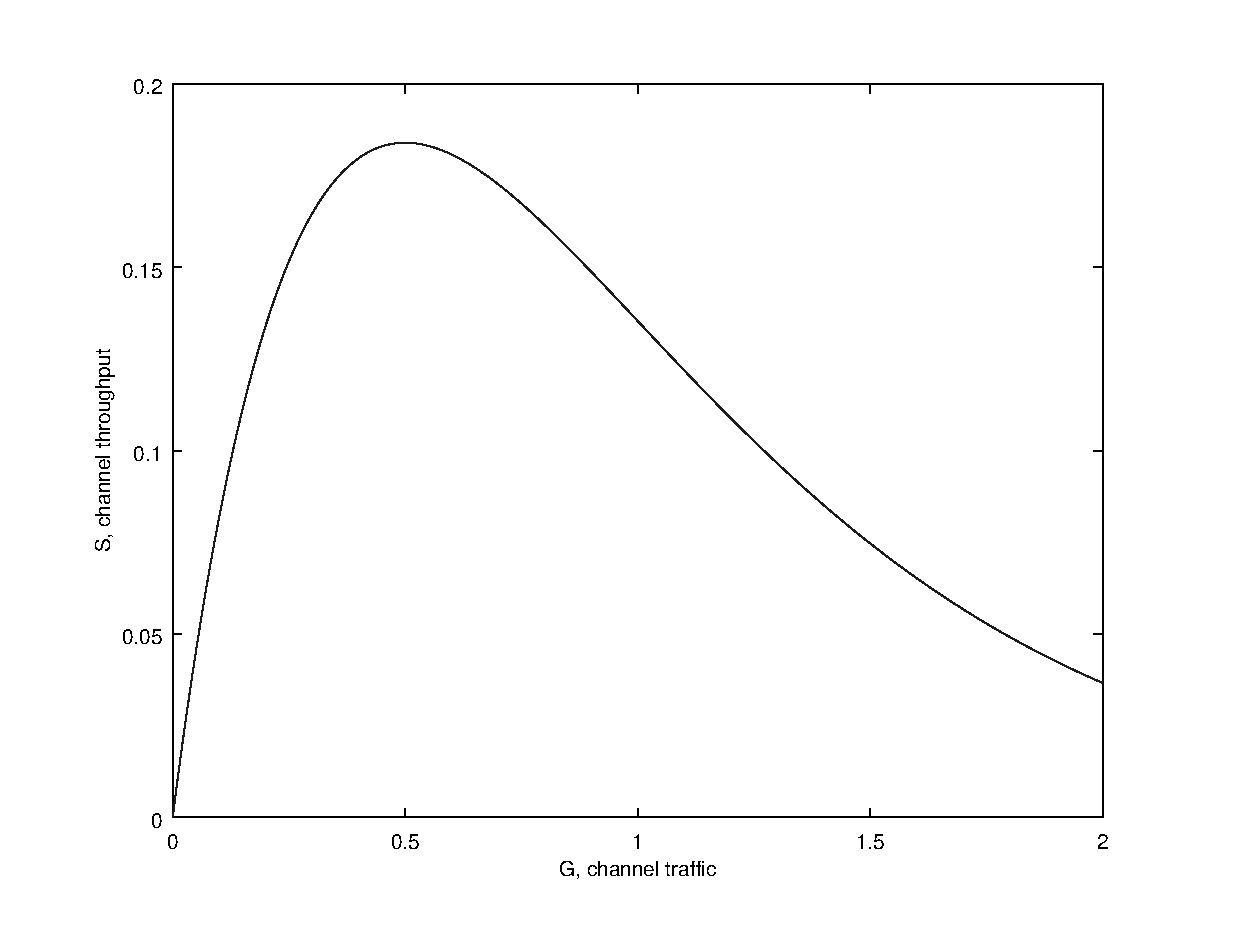
\includegraphics[width=1.0\textwidth]{src/octave/poissonthroughput}
	\caption{Poisson channel traffic and throughput}
	\label{fig:SGpoisson}
\end{figure}
Graphing the channel throughput versus the channel's traffic yields figure 
\ref{fig:SGpoisson}, which indicates that as you increase channel traffic, 
throughput increases to an inflection point when there is no unused channel capacity
and packet collisions finally start to dominate
the channel and harm throughput. This inflection point happens to be at
an incoming traffic $G = 0.5$ which yields an expectation that 36\% of the packets
will be successfully received ($S = 0.18$).

While assuming that APRS traffic is based on a Poisson process is 
highly suspect, this simple model of channel capacity does yield some insightful 
values. 
Collecting several days of APRS traffic on 144.390MHz in San Luis Obispo, California
shows an average packet size of 119 octets. With a typical 300ms preamble,
the assumption that every packet is the mean length,
and a data rate of 1200bps, this yields $\tau = 1.09$ seconds.
\begin{equation}
	\lambda_{APRS} = \frac{G_{MAX}}{\tau} = 0.457
	\label{equ:aprsmaxrate}
\end{equation}

Equation \ref{equ:aprsmaxrate} indicates that a single APRS channel can support
0.457 transmitted packets per second, or
27 packets per minute, which need to be shared between
all of the participating network nodes.
Assuming the typical target LAN size of 60 stations, 
this implies an average packet interval per station
of \emph{2 minutes 13 seconds}.\footnote{For the reader skimming this chapter, DO NOT
	use this beacon interval for APRS; this Poisson model is too simplified to give
meaningful results. A suggested default is 600 second intervals.}
The less satisfying result is the fact that only 10 of these packets every minute will be
successful received, which indicates that
two thirds of the transmitted power is wasted.

The next section will go into how this Poisson model is deficient to the
point that this 2 minute 13 seconds value is nearly meaningless.
Any station that beaconed that fast on an actual APRS network could very quickly
be identified as abusive to the rest of the network, so further work is needed
before an analytic interval suggestion can be made.
What this calculation does demonstrate is that the general concept of 60 stations
sharing a single ALOHA channel in the way APRS intends is within the realhm of
possibilities. 
Had this value come out an order of magnitude larger, the claim
that APRS could allow a user to discover 60 other stations would be much more suspect.

\section{Deficiencies of the Poisson Model}

There were several assumptions made to simplify the just-presented model 
for an ALOHA channel that are not particularly valid 
when applied to a typical APRS network. 
While most of these assumptions indicate that the result of
equation \ref{equ:aprsmaxrate} is overly optimistic and 
stations should beacon less often, there are enough different mechanisms at play
in both directions that the true traffic versus throughput relationship 
is not easily found and requires further work beyond this paper.
Some of the ignored issues include:

\begin{itemize}
	\item Differences in packet length -- Actual APRS traffic varies in length,
		which has an effect on throughput rates by changing $\tau$.
		Abramson considered the general
		case for two discrete packet lengths \cite{packetthroughput},
		but in general this encourages users to make packets as short as possible
		to improve throughput.
	\item Digipeaters and channel access methods -- The presented model assumes that
		every packet is added to the channel as an entirely blind shot in the dark,
		but many APRS stations use CSMA to avoid transmitting on already busy channels.
		This reduces the window for destructive collisions and thus reduces the ratio
		between the channel traffic G and the usable throughput S.
	\item Sources of entropy in the network -- Starting with a Poisson stocastic model
		implies a strong assumption that every packet starts at a random time independent
		of every other packet. Many APRS stations beacon on a fixed interval,
		such as 600 seconds, which makes that station's traffic very self-similar.
		Digipeaters also strongly break this assumption by their action of immediately
		repeating packets after they're originally transmitted.
		These digipeater echos aren't random at all.
		Papers have been written on the misuse of poisson traffic models with regards
		to TCP/IP networks \cite{failureofpoisson}, and those arguments often apply
		equally well to the APRS network.
	\item The heterogeneous nature of APRS equipment -- Any closed-form analysis
		of APRS depends on each network node behaving in one of a small set 
		of possible behaviors. The home-brewed and come-as-you-are nature of APRS
		makes the cumulative behavior of the network at large much harder to model.
		Useful models would need to depend on careful measurement of the behavior of
		existing nodes, and likely use Monte Carlo methods to make meaningful
		statements about the system at large.
\end{itemize}

In the end, building a meaningful model for APRS network traffic will likely prove
to be surprisingly challenging.
Much of this derives from the unusual amount of latitude given to APRS implementations
by the lack of detailed specifications that causes the aggregate network to behave so
unpredictably.
For further work modeling APRS to deliver meaningful results,
it's likely that it will need to begin by making a decision on which existing nodes in the
APRS network are ``misbehaving" by some developed metric and exclude them from
any further analysis.

The community has been extremely reluctant to outright classify APRS hardware
as misbehaving in the past,
due to the embedded nature of APRS nodes that usually precludes any major
modifications in behavior of existing nodes.
Classitying a node as misbehaving often meant that the operator would need to
spend a significant amount of time and money outright replacing the deficient hardware.
As more APRS nodes move to open-source and/or reprogramable implementations,
it's conceivable that updates to APRS behavior as resulting 
from future research may become merely difficult,
instead of utterly impossible.\footnote{For example, the open source aprx package is
	one of the most popular pieces of i-gate software on the network \cite{aprxpopular},
	and modern trackers like those from Argent Data often
enjoy firmware updates which are relatively easy to install.}





\end{document}
